\section{AAR}

AAR is an important timing consideration in the Mission Plan. The timing must
coincide with other flights, On station time, VUL windows and the overall
mission plan for maximum effect. Don't be caught at the back of the queue.

Many flights are late to their mission due to poor anticipation of the length
of time AAR can take, especially with trickier handling airframes, wake
turbulence, control issues, lack of practice and queues behind other flights,
not to mention unexpected DCS behaviour AKA "Tanker dogfighting". Preplanned
AAR will not need an agency check-in request, however, on Station AAR will
cause a gap in defences, usually at an inopportune time for the AIC coverage.
Make sure to request and plan  leaving station for AAR and keep ahead of the
Flight's fuel status.

\subsection{Process}

The flight leader should ahead of time prioritise any flight member with
significantly lower fuel in the flight and place them ahead of the order of
planes in left echelon. The detachment will close from 1000 feet beneath and
aft of the tanker to visually ensure a clear space to take the observation
area. The flight will form up in the observation area. One at a time from the
inside out, pilots will request refuelling for as many hoses as exist on the
tanker type.

\sidebyside{0.45}{

  After refuelling the Flight should form up on the tanker's right wing in
  order. Note that only one aircraft may change position at any one time. This
  reduces the risk of in-air collisions.

  The order of aircraft on the tanker's right wing after refuelling may be
  reversed by lead if the situation justifies, for example if the flight will
  peel off right immediately after.

  Tomcat's may find forcing the Wingsweep to \textbf{Bomb mode} easier to
  maintain constant speed.

  Tomcat's should \textbf{avoid Speed brakes} in formation as they come with
  dramatic drops in altitude.

  NB. Tomcat has two settings for refuelling, Internal only and Internal +
  Tanks. Be aware which one has been selected.
}{%
  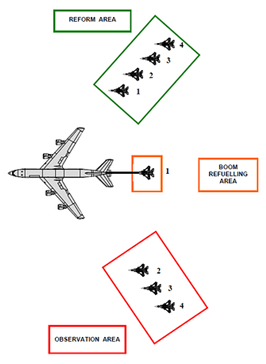
\includegraphics[width=\textwidth,align=t]{aar/layout2}%
}
